\mychapter{Ambiente de Execução}
\label{Cap:Ambiente de Execução}

\section{Introdução}
O trabalho feito até agora visava mais o reconhecimento de uma linguagem compilada, sendo portanto um processo comum para o desenvolvimento de todo e qualquer compilador podendo ser repetida para qualquer nova linguagem independente da linguagem "alvo" (gerada pela compilação). Entretanto, sendo esse um trabalho de um compilador, cedo ou tarde é necessário estudar a linguagem gerada, se ainda não escolhida.

No caso, o código gerado será utilizada para a máquina disponibilizada, MVN (Máquina de Von Neumann)\cite{mvn_implementation}, que simula um processador simples composto de Memória, Acumulador e Registradores Auxiliadores.

A linguagem de saída do compilador desenvolvido utiliza uma linguagem simbólica de mnemônicos descrita nos itens \ref{sec:instrucoes} e  \ref{sec:pseudoinstrucoes}. A linguagem de saída é assim construída para utilizar o Montador disponibilizado, que também faz parte do ambiente de execução.

\section{Instruções da linguagem de saída}
\label{sec:instrucoes}
A listagem e descrição das instruções da linguagem de saída se encontram na tabela \ref{tab:tabela-instrucoes}
\begin{table}
\centering{
\renewcommand{\tabcolsep}{0.2cm}
\begin{tabular}{|L{2cm}|l|L{4cm}|L{4cm}|}
\hline
\textbf{Operação} & \textbf{Mnem.} & \textbf{Operando} & \textbf{Descrição} \\
\hline
Jump & JP & Endereço ou Rótulo de desvio & Desvio incondicional \\
\hline
Jump if Zero & JZ & Endereço ou Rótulo de desvio & Desvio se acumulador é zero \\
\hline
Jump if Negative & JN & Endereço ou Rótulo de desvio & Desvio acumulador é negativo \\
\hline
Load Value & LV & Constante de 12 bits & Carrega uma constante no acumulador \\
\hline
Add & + & Endereço ou Rótulo da parcela & Soma do acumulador com a parcela \\
\hline
Subtract & - & Endereço ou Rótulo do subtraendo & Subtração do acumulador com o subtraendo \\
\hline
Multiply & * & Endereço ou Rótulo do multiplicador & Multiplicação do acumulador com o multiplicador \\
\hline
Divide & / & Endereço ou Rótulo do divisor & Divisão do acumulador com o divisor \\
\hline
Load & LD & Endereço ou Rótulo do dado & Carrega valor contido no endereço de memória para acumulador \\
\hline
Move to Memory & MM & Endereço ou Rótulo de destino do dado & Carrega valor do acumulador para a memória \\
\hline
Subroutine Call & SC & Endereço ou Rótulo do subprograma & Desvio para subprograma \\
\hline
Return from Subroutine & RS & Endereço ou Rótulo de retorno & Retorno de subprograma \\
\hline
Halt Machine & HM & Endereço ou Rótulo do desvio & Parada \\
\hline
Get Data & GD & Dispositivo de E/S & Entrada \\
\hline
Put Data & PD & Dispositivo de E/S & Saída \\
\hline
Operating System & OS & Constante & Chamada de supervisor \\
\hline
\end{tabular}}
\caption{\label{tab:tabela-instrucoes} Tabela de instruções.}
\end{table}

\section{Pseudoinstruções da linguagem de saída}
\label{sec:pseudoinstrucoes}
A listagem e descrição das pseudoinstruções da linguagem de saída se encontram na tabela \ref{tab:tabela-pseudoinstrucoes}
\begin{table}
\centering{
\renewcommand{\tabcolsep}{0.2cm}
\begin{tabular}{|l|L{11cm}|}
\hline
\textbf{Pseud.} & \textbf{Descrição} \\
\hline
@ & Recebe um operando numérico, define o endereço da instrução seguinte \\
\hline
K & Reserva uma área para constante de 2 bytes (operando hexadecimal) \\
\hline
\$ & Reserva uma área de dados com tamanho especificado (operando hexadecimal) \\
\hline
\# & Define o fim físico do texto-fonte \\
\hline
\& & Define uma origem relocável para o código a ser gerado, o operando é o endereço em que o próximo código se localizará (relativo à origem do código atual) \\
\hline
> & Define endereço simbólico de entrada (Entry Point) \\
\hline
< & Define um endereço simbólico que referencia um entry-point externo (External) \\
\hline
\end{tabular}}
\caption{\label{tab:tabela-pseudoinstrucoes} Tabela de pseudoinstruções.}
\end{table}

\section{Características Gerais}
O simulador em questão apresenta algumas caracteríscas que devem ser levadas em conta para um melhor entendimento dele:

\begin{figure}[H]
\centering
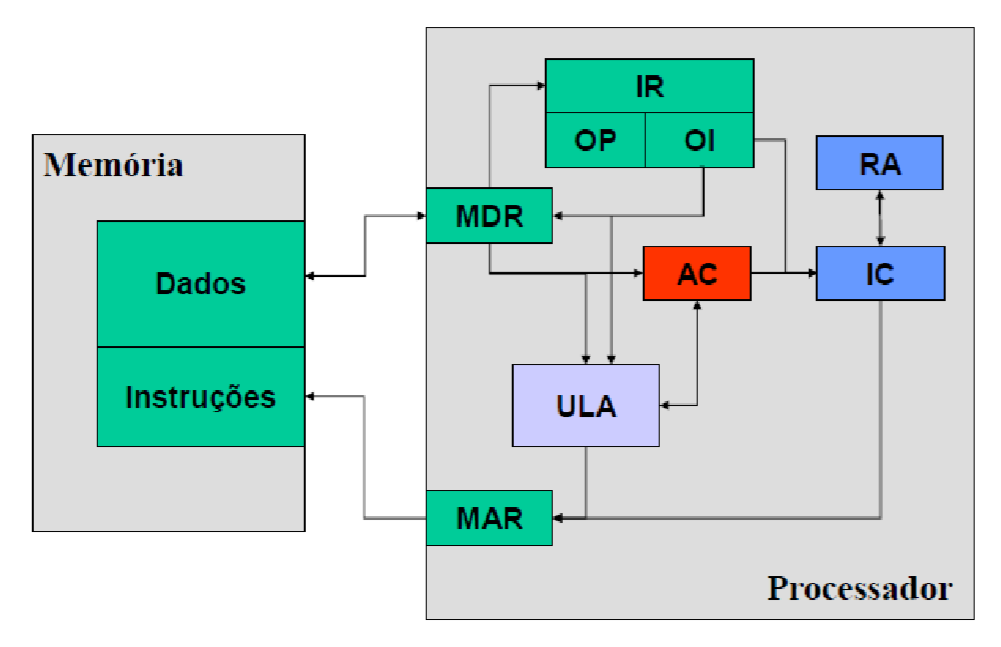
\includegraphics[width=8cm,keepaspectratio]{figuras/mvn.png}
\caption{\label{fig:mvn} arquitetura da MVN disponibilizada}
\end{figure}

\begin{itemize}
  \item{O ambiente de execução é composto por um simulador com: memória principal, acumulador e registradores auxiliares;}

  \item{Arquitetura de Von Neumann: área de memória compartilhada entre código e dados;}

  \item{Arquitetura de acumulador: apesar de apresentar utilizar alguns registradores, apenas um está disponível para uso do programador, com exceção dos registradores de instrução (que sempre deve poder ser configurado pelo indivíduo): o acumulador. Logo, o manuseio de dados conta com vários acessos à memória;}
  
  \item{Words de 2 bytes/quatro hexas: tanto para instruções quanto para dados, sendo, no caso de instruções, o primeiro valor hexa reservado para identificar a instrução. Isso implica e explica a existência das 16 operações já explanadas e memória com 4095 words de tamanho (item seguinte);}
  
  \item{Memória com 4095 words (0xFFF) de tamanho: Uma vez que deve ser possível apontar para todos os endereços de memória para realizar operações de memória, não faz sentido ter mais que tal espaço;}
  
  \item{Endereçamento por bytes: Apesar de uma word formar uma instrução, muitas vezes deseja-se trabalhar com dados em forma de bytes, por isso o endereçamento de memória é feito por bytes, o que também pode gerar um certo estranhamento quando a primeira instrução ocorre no espaço zero e a segunda instrução no dois. É apenas o efeito de uma decisão de projeto}
  
  \item{Operações aritméticas básicas, apenas: todas as operações devem ser realizadas com operações aritméticas. Caso a linguagem compilada entenda operadores lógicos, esses devem ser implementados com operações  aritméticas;}
  
  \item{Implementação de subrotinas: O simulador já possui uma implementação para auxiliar o uso e construção de subrotinas. Ao usar a chamada de SC, o valor de endereço "mais um" é guardado no início da subrotina e para retornar usando RS, esse endereço guardado na chamada de SC é usado para retornar. Essa implementação gera o problema de funções recursivas, uma vez que a função, ao chamar a sí mesma iria perder a referência ao programa principal. Para contornar esse problema, deve-se implementar um trecho de código auto-modificável ou uma pilha, o que apresenta um outro grande problema: devido à memória reduzida da máquina, dependendo da profundidade da recursão, o programa pode acabar usando muita memória para a pilha;}
  
  \item{Memória reduzida: como mencionado acima, devido à memória limitada, em muitos trechos deve-se usar da auto-modificação de código para conservar memória, um artifício considerado "sujo" porém eficiente, dependendo do programador, mas que ofusca muito o código para leitores terceiros;}
  
  \item{Pseudo-comandos para a modularização do código final e reserva de espaço: Apesar de não funcionais (não possuem uma função no código em sí), a MVN implementa cinco pseudo símbolos que auxiliam na modularização, ao possibilitar a separação do código em arquivos com a idéia de importação e exportação de símbolos e endereços relativos para que não seja necessário calcular o endereço de cada instrução na memória, e o gerenciamento de memória, como a declaração de constantes, valores que não devem mudar durante a execução do programa, e blocos de memória, que reservam um grande bloco de bytes de uma vez;}
  
\end{itemize}
